\documentclass[a4paper, 11pt]{article}


\usepackage[slovak, czech]{babel}
\usepackage[utf8]{inputenc}
\usepackage[left=2cm, top=3cm, text={17cm, 24cm}]{geometry}
\usepackage[T1]{fontenc}
\usepackage{times}
\usepackage{verbatim}
\usepackage{enumitem}
\usepackage{graphicx} 
\usepackage[unicode]{hyperref}
\usepackage{hyperref}
\usepackage{listings}
\usepackage{color}

\definecolor{dkgreen}{rgb}{0,0.6,0}
\definecolor{gray}{rgb}{0.5,0.5,0.5}
\definecolor{mauve}{rgb}{0.58,0,0.82}

\lstset{language=SQL,
  aboveskip=3mm,
  belowskip=3mm,
  showstringspaces=false,
  columns=flexible,
  basicstyle={\small\ttfamily},
  numbers=none,
  numberstyle=\tiny\color{gray},
  keywordstyle=\color{blue},
  commentstyle=\color{dkgreen},
  stringstyle=\color{mauve},
  breaklines=true,
  breakatwhitespace=true,
  tabsize=3
}



\begin{document}
\begin{titlepage}
		\begin{center}
			
\includegraphics[width=0.77 \linewidth]{FIT_logo.pdf} \\

			\vspace{\stretch{0.382}}

			\Huge{Projekt 5. časť} \\
			\Huge{Projektová dokumentácia} \\
			\LARGE{\textbf{Zoologická záhrada}} \\
			\Large{Databázové systémy}

			\vspace{\stretch{0.618}}
		\end{center}

		{\Large
			\today
			\hfill
			\begin{tabular}{ll}
			Samuel Dobroň & \href{mailto:xdobro23@stud.fit.vutbr.cz}{\texttt{xdobro23@stud.fit.vutbr.cz}} \\
            Juraj Remeň & \href{mailto:xremen02@stud.fit.vutbr.cz}{\texttt{xremen02@stud.fit.vutbr.cz}}
\end{tabular}
}
	\end{titlepage}
	\newpage
	\tableofcontents
	\newpage
	\section{Zadanie}
	Navrhněte informační systém pro zoologickou zahradu. V zoologické zahradě jsou živočichové umístěni do klecí, výběhů, či do klecí v pavilonech. Živočichové jsou děleni podle třídy, řádu, čeledě, rodu a druhu (např. lama alpaka je v třídě savců, řádu sudokopytníků, v čeledi velbloudovitých, v rodu lama a druhu alpaka). Pro zjednodušení předpokládejte striktně hierarchické dělení živočichů a to, že každý živočich je příslušníkem právě jednoho druhu. Jeden druh živočicha může být v několika výbězích či klecích, a naopak, v jednom výběhu či kleci může být více různých druhů. Systém musí být schopný vyhledávat živočichy podle jejich příslušností do jednotlivých kategorií. Pro každého živočicha je třeba uchovávat informace o datu narození (a případně úmrtí), jméno, historii výsledků měření (hmotnosti, rozměrů, ...), apod.
	\section{Implementácia}
	\subsection{Úvod}
	Naša implementácia začala vytvorením tabuliek, ktoré odzrkadľovali návrh v~podobe ER diagramu. Nasledovalo určenie primárnych kľúčov tabuliek, cudzích kľúčov a vytváranie tabuliek, ktoré zobrazovali vzťahy medzi entitami v~ER diagrame. Po vytvorení tabuliek sme ich naplnili ukážkovými dátami.\\
	\par Ďalšou fázou bolo vytvorenie SELECT dotazov, uvádzame len pár z nich, všetky ostatné sú okomentované a uvedené v kóde.
	\subsubsection{Spojenie 2 tabuliek príkazom SELECT}
	Vypíše meno, priezvisko, nazov pozicie a náplň práce zamestnanca:
	 \begin{lstlisting}
    SELECT meno, priezvisko, nazov, napln_prace FROM zamestnanec NATURAL JOIN pozicia WHERE pozicia.ID_pozicie = zamestnanec.pozicia;
  	 \end{lstlisting}

	\subsubsection{Spojenie 3 tabuliek príkazom SELECT}
	Vypíše mená živočíchov, kde sú umiestnené a o aký typ umiestnenia ide:
	\begin{lstlisting}
    SELECT meno, nazov, CASE WHEN interakcia is not null THEN 'Vybeh' ELSE 'Pavilon' END AS Typ_umiestnenia FROM zivocich NATURAL JOIN bol_umiestneny NATURAL JOIN umiestnenie;
    	\end{lstlisting}
    	
    \subsubsection{SELECT s použitím EXISTS}
    Vypíše ID, mená a priezviská zamestnancov, ktorí neošetrujú žiadne zviera:
    \begin{lstlisting}
    SELECT ID_zamestnanca, meno, priezvisko FROM zamestnanec Z WHERE NOT EXISTS(SELECT * FROM osetruje WHERE osetruje.ID_zamestnanca = Z.ID_zamestnanca);
    \end{lstlisting}


	\subsection{Generalizácia}
	Pri vytváraní vzťahu generalizácie sme použili jednu tabuľku nadtypu \texttt{UMIESTNENIE}, v ktorej podľa istého kritéria, v našom prípade ide o možnosť interakcie so zvieratami, rozlišujeme o aký typ umiestenia ide.
	\subsection{EXPLAIN PLAN a použitie INDEX}
    Úlohou \texttt{EXPLAIN PLAN} je zobrazenie postupnosti operácií za pomoci optimalizátorov.
        \subsubsection{Naša implementácia príkazu EXPLAIN PLAN}
    Na základe poskytnutých dát o cene a čase jednotlivých operácií sme si vybrali, tabuľkové hodnoty bude najlepšie optimalizovať.
    
    \begin{lstlisting}
    EXPLAIN PLAN FOR
SELECT Z.ID_zivocicha, Z.meno, COUNT(*) osetrovatelov
FROM zivocich Z
NATURAL JOIN
    typ_zivocicha T,
    vlastnost V,
    osetruje O
WHERE T.ID_triedy = 1
    AND V.ID_vlastnosti = 1
    AND V.ID_zivocicha = Z.ID_zivocicha
    AND Z.ID_zivocicha = O.ID_zivocicha
    AND hodnota > 100
GROUP BY Z.ID_zivocicha, meno
HAVING COUNT(O.ID_zamestnanca) < 3;
SELECT PLAN_TABLE_OUTPUT FROM TABLE(DBMS_XPLAN.DISPLAY());
    \end{lstlisting}
    Po zavolaní príkazu \texttt{EXPLAIN PLAN} a vypísaní na výstup, je možné vidieť tabuľku s postupnosťou vykonávaných operácií a taktiež ich výkonnostnú cenu.
	\begin{figure}[h]
	\scalebox{0.6}{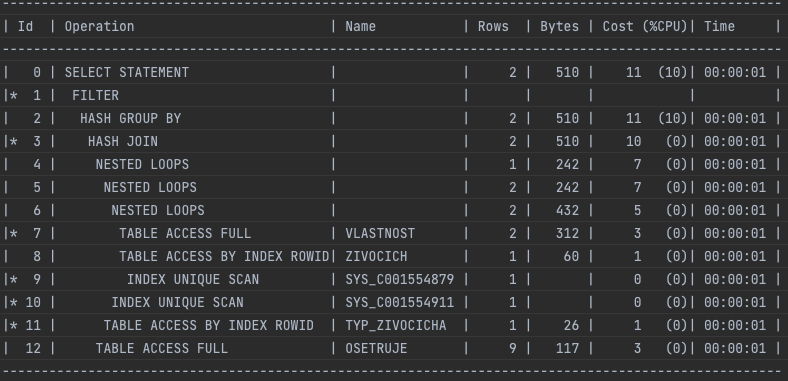
\includegraphics{plan_wo_index.png}}
	\centering
	\caption{EXPLAIN PLAN bez použitia indexov}
	\end{figure}
\newpage
        \subsubsection{INDEX}
         K~urýchleniu prevedenia príkazu bol pridaný \texttt{INDEX} nakoľko indexovanie môže byť užitočné v~prípade častého vyhľadávania v~určitej tabuľke. V~našej implementácií často používame tabuľky \texttt{TYP\_ZIVOCICHA}, \texttt{OSETRUJE}, \texttt{VLASTNOST} a \texttt{ZIVOCICH}.
          Preto sme implementovali príkazy \texttt{INDEX} nasledovne:
    \begin{lstlisting}
    CREATE INDEX trieda_index ON typ_zivocicha(ID_triedy);
    CREATE INDEX vlastnost_index ON vlastnost(ID_zivocicha, ID_vlastnosti, hodnota);
    CREATE INDEX osetruje_index ON osetruje(ID_zivocicha);
    \end{lstlisting}
        Pri druhom spustení príkazov s~EXPLAIN PLAN za použitia indexov je viditeľné, že operácie sa vykonali rýchlejšie s~menšou výkonnostnou cenou. Taktiež miesto prechodu celou tabuľkou bolo zvolené skenovanie indexov. Táto zmena zabezpečila rýchlejšie/nenáročnejšie vykonanie väčšiny operácií v rámci príkazu.
	
	\begin{figure}[h]
		\scalebox{0.6}{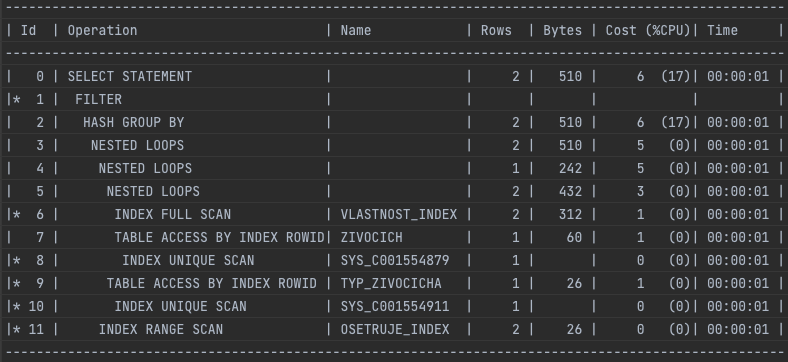
\includegraphics{plan_w_index.png}}
		\centering
		\caption{EXPLAIN PLAN s použitím indexov}
	\end{figure}

	\subsection{Procedúry} 
	V~skripte sú implementované dve procedúry:\\
	\texttt{kompletny\_prehlad()}\\
	\texttt{obsadenost(potrebna\_plocha\_param, typ\_umiestnenia)}
	
	Procedúra \texttt{kompletny\_prehlad()} vypíše aktuálny počet živých alebo mŕtvych zvierat v databáze, priemerný počet zvierat v jednotlivom umietnení a priemerný počet zvierat na ošetrovateľa. Procedúra nepríjma žiadne parametre. Vypočíta potrebné premenné pomocou agregačnej funkcie \texttt{COUNT} a pomocou nich prepočíta priemery a sumy. Na DBMS výstup neskôr vypíše tieto údaje. V prípade, že by hodnota počtu umiestnení, alebo počtu ošetrovateľov mala byť rovná 0, tak sa vyvolá výnimka.
	
	Procedúra \texttt{obsadenost(potrebna\_plocha\_param, typ\_umiestnenia)} vypíše percentuálnu obsadenosť typu umiestnenia podľa zadanej priemernej potrebnej životnej plochy a typu umiestnenia. Táto informácia je potrebná v prípade obstarania nových zvierat. Procedúra príjma 2 parametre od užívateľa. V prípade chybného vstupu sa vyvolá výnimka. Procedúra prechádza všetkými umiesteniami v databáze a na základe užívateľom zadaného typu vypočíta celkovú využiteľnú plochu daného typu umiestnenia a počet zvierat umiestnených v danom type. Na DBMS výstup neskôr vypíše celkovú percentuálnu obsadenosť typu umiestnenia. V prípade, že by sa celková plocha umiestnenia rovnala 0, tak opäť výnimku vyvolá.
	
	\subsection{Triggre}
	V~skripte sú implementované dva triggre: \\
	\texttt{"pochovaj\_zviera"}\\
	\texttt{"zahashuj\_heslo"}\\
	
	Trigger \texttt{"pochovaj\_zviera"} má za úlohu nastaviť dobu \textbf{do} v \texttt{bol\_umiestneny} pri zadaní dátumu úmrtia zvieraťa do databázy a odstrániť jeho ošetrovateľa v \texttt{osetruje}. Zároveň má za úlohu aj kontrolu validity dátumu úmrtia, v prípade, že je dátum úmrtia starší ako dátum narodenia sa vyvolá výnimka.\\
	
	Trigger \texttt{"zahashuj\_heslo"} má za úlohu zahashovať zadané \textbf{heslo} v \texttt{zamestanec} použije funkciu \texttt{MD5()} z knižnice \texttt{DMBS\_OBFUSCATION\_TOOLKIT} a nami zadaného \textbf{saltu}.
	
	\subsection{Materializovaný pohľad}
	Je to objekt, ktorý poskytuje dáta v~rovnakej podobe ako tabuľka. Narozdiel od tabuľky, ktorá obsahuje priamo dáta, pohľad obsahuje len predpis akým spôsobom dáta získať z~iných tabuliek alebo pohľadov. Materializovaný pohľad sa uloží a predspracuje, čo neplatí o~nematerializovanom pohľade.\\
	\par Náš materializovaný pohľad vytvára tabuľku \texttt{pocet\_zivocichov\_v\_umiestneniach}, ktorá vytvára dáta, konkrétne počet živočíchov v jednotlivých pavilónoch a výbehoch.

	\subsection{Práva}
	Pomocou príkazu GRANT na tabuľky nasledovaný zoznamom práv, ktoré chceme udeliť, zvolili sme príkaz ALL (všetky práva), nasledovaný názvom tabuliek, ku ktorým chceme pristupovať a udeliť práva (všetky tabuľky a materializované pohľady) a nakoniec treba uviesť, komu sa tieto práva udeľujú, čo v~našom prípade bol kolega \textit{xremen02}.

	\section{Záver}
	Pri vypracovaní projektu sme nemali žiadne závažné problémy v~komunikácii, keďže sme spolubývajúci a vždy sme sa dohodli na kontrétnom dni a hodine kedy a o koľkej budeme na projekte pracovať. Na komunikáciu sme používali Discord a osobné stretnutia. Na verzovanie projektu sme využili systém Github pre ľahšiu orientáciu. Všetky projekty sme vypracovávali v predstihu, aby sme sa vyhli stresu a nervozite z preťaženia servera. Vývoj projektu prebiehal na školskom serveri a v~prostredí od JetBrains \-- Data Grip. Pri vypracovávaní sme využili aj menšiu konzultáciu s pedagógmi.
\end{document}